%=====================================================================
% Table Name Cheat-Sheet
%
% Programmer	:	ABOUZAR KABOUDIAN
% Date			:	2016-08-03
% Place			: 	Gergia Institute of Technology
%=====================================================================
\documentclass[tikz, border=10pt]{standalone}
\usepackage{verbatim}
\usepackage{amssymb}
\usetikzlibrary{shapes.callouts}
\tikzset{
  level/.style   = { ultra thick, blue },
  connect/.style = { thick, red },
  notice/.style  = { draw, rectangle callout, callout relative pointer={#1} },
  label/.style   = { text width=2cm }
}


\newcounter{rowNo}
\newcounter{colNo}
\newcommand{\x}{7.*\arabic{colNo}}
\newcommand{\y}{-2.5*\arabic{rowNo}}
\newcommand{\newRow}{\stepcounter{rowNo}}

% Channel name and corresponding channels
% \shader{texture name}
%	{r-channel}
%	{g-channel}
%	{b-channel}
%	{a-channel}
\newcommand{\newColumn}{\setcounter{rowNo}{0}\stepcounter{colNo}}

\newcommand{\shader}[5]{
	\newRow
	\node[label] at (\x-.3,\y)  {\texttt{#1}} ;
	\draw[connect,color=red] (\x,\y) -- (\x+1,\y+1);
	\draw[connect,color=green] (\x,\y) -- (\x+1,\y+0.5);
	\draw[connect,color=blue] (\x,\y) -- (\x+1,\y);
	\draw[connect,color=yellow] (\x,\y) -- (\x+1,\y-.5);
	\node[label] at (\x+2.1,\y+1)  {$#2$} ;
	\node[label] at (\x+2.1,\y+0.5)  {$#3$} ;
	\node[label] at (\x+2.1,\y)  {$#4$} ;
	\node[label] at (\x+2.1,\y-.5)  {$#5$} ;	
}


\newcommand{\checked}[1]{
	\if#11
		{$\checkmark$}
	\else
		{\ }	
	\fi
}

\newcommand{\finished}[1]{
	\if#11
	{$\dag$}
	\else
	{\ }	
	\fi
}
\newcommand{\dble}[1]{
	\if#11
	{$-$}
	\else 
		\if#12
			{$+$}
		\else
			{\ }	
		\fi
	\fi
}


\newcommand{\xcchShift}{4.5}
\newcommand{\finishedChannel}[4]{
	\node[label] at (\x+\xcchShift,\y+1)  {\finished{#1}};
	\node[label] at (\x+\xcchShift,\y+0.5)  {\finished{#2}} ;
	\node[label] at (\x+\xcchShift,\y)  {\finished{#3}} ;
	\node[label] at (\x+\xcchShift,\y-.5)  {\finished{#4}} ;
}

\newcommand{\xchShift}{4.8}
\newcommand{\checkedChannel}[4]{
	\node[label] at (\x+\xchShift,\y+1)  {\checked{#1}};
	\node[label] at (\x+\xchShift,\y+0.5)  {\checked{#2}} ;
	\node[label] at (\x+\xchShift,\y)  {\checked{#3}} ;
	\node[label] at (\x+\xchShift,\y-.5)  {\checked{#4}} ;
}

\newcommand{\xdchShift}{5.1}
\newcommand{\dCheckChannel}[4]{
	\node[label] at (\x+\xdchShift,\y+1)  {\dble{#1}};
	\node[label] at (\x+\xdchShift,\y+0.5)  {\dble{#2}} ;
	\node[label] at (\x+\xdchShift,\y)  {\dble{#3}} ;
	\node[label] at (\x+\xdchShift,\y-.5)  {\dble{#4}} ;
}
\newcommand{\txt}[1]{\mbox{\scriptsize #1}}
\newcommand{\utxt}[1]{_{\txt{#1}}}
\newcommand{\ion}[1]{[\mbox{#1}]}

%@@@@@@@@@@@@@@@@@@@@@@@@@@@@@@@@@@@@@@@@@@@@@@@@@@@@@@@@@@@@@@@@@@@@@
% Document begins
%@@@@@@@@@@@@@@@@@@@@@@@@@@@@@@@@@@@@@@@@@@@@@@@@@@@@@@@@@@@@@@@@@@@@@
\begin{document}
	
%=====================================================================
% Tikz picture environment
%=====================================================================
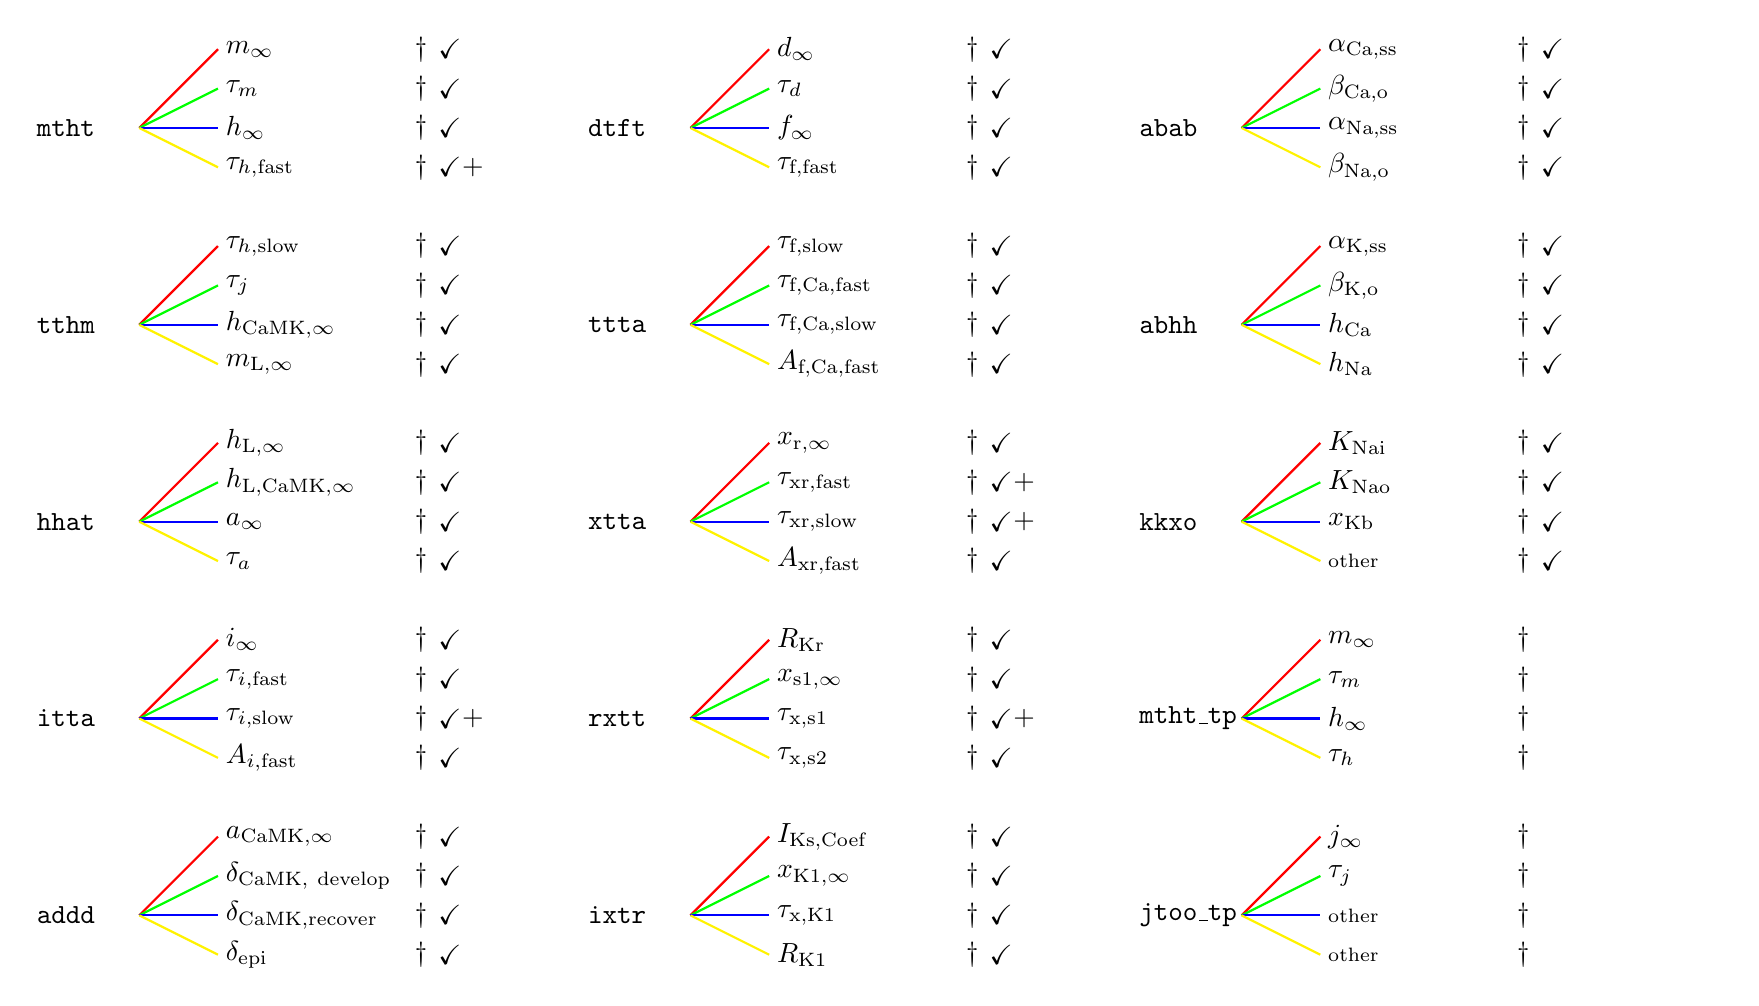
\begin{tikzpicture}				    
%---------------------------------------------------------------------
% First Column
%---------------------------------------------------------------------
	\shader{mtht}
		{m_\infty}
		{\tau_m}
		{h_\infty}
 		{\tau_{h,\txt{fast}}} 	
 	\finishedChannel{1}{1}{1}{1}
 	\checkedChannel{1}{1}{1}{1}
 	\dCheckChannel{0}{0}{0}{2}
 	
	\shader{tthm}
		{\tau_{h,\txt{slow}}}
		{\tau_j}
		{h_{\txt{CaMK},\infty}}
		{m_{\txt{L},\infty}}
	\finishedChannel{1}{1}{1}{1}
	\checkedChannel{1}{1}{1}{1}
		
	\shader{hhat}
		{h_{\txt{L}, \infty}}
		{h_{\txt{L,CaMK},\infty}}
		{a_\infty}{\tau_a}
	\finishedChannel{1}{1}{1}{1}
	\checkedChannel{1}{1}{1}{1}
		
	\shader{itta}
		{i_\infty}
		{\tau_{i,\txt{fast}}}
		{\tau_{i,\txt{slow}}}
		{A_{i,\txt{fast}}}
	\finishedChannel{1}{1}{1}{1}
	\checkedChannel{1}{1}{1}{1}
	\dCheckChannel{0}{0}{2}{0}
	
	\shader{addd}
		{a_{\txt{CaMK},\infty}}
		{\delta\utxt{CaMK, develop}}
		{\delta\utxt{CaMK,recover}}
		{\delta\utxt{epi}}
	\finishedChannel{1}{1}{1}{1}
	\checkedChannel{1}{1}{1}{1}
	
%---------------------------------------------------------------------
% Second Column
%-------------------------------------------------------------------
	\newColumn
	\shader{dtft}
		{d_\infty}
		{\tau_d}
		{f_\infty}
		{\tau\utxt{f,fast}}
	\finishedChannel{1}{1}{1}{1}
	\checkedChannel{1}{1}{1}{1}
	\dCheckChannel{0}{0}{0}{0}
	
	\shader{ttta}
		{\tau_{\txt{f,slow}}}
		{\tau_{\txt{f,Ca,fast}}}
		{\tau\utxt{f,Ca,slow}}
		{A\utxt{f,Ca,fast}}
	\finishedChannel{1}{1}{1}{1}
	\checkedChannel{1}{1}{1}{1}
	\dCheckChannel{0}{0}{0}{0}	
		
	\shader{xtta}
		{x_{\txt{r},\infty}}
		{\tau\utxt{xr,fast}}
		{\tau\utxt{xr,slow}}
		{A\utxt{xr,fast}}
	\finishedChannel{1}{1}{1}{1}
	\checkedChannel{1}{1}{1}{1}
	\dCheckChannel{0}{2}{2}{0}	
			
	\shader{rxtt}
		{R\utxt{Kr}}
		{x_{\txt{s1},\infty}}
		{\tau\utxt{x,s1}}
		{\tau\utxt{x,s2}}
	\finishedChannel{1}{1}{1}{1}
	\checkedChannel{1}{1}{1}{1}
	\dCheckChannel{0}{0}{2}{0}
	
	\shader{ixtr}
		{I\utxt{Ks,Coef}}
		{x_{\txt{K1},\infty}}
		{\tau\utxt{x,K1}}
		{R\utxt{K1}}
	\finishedChannel{1}{1}{1}{1}
	\checkedChannel{1}{1}{1}{1}
	\dCheckChannel{0}{0}{0}{0}
	
%---------------------------------------------------------------------
% Third Column
%---------------------------------------------------------------------
	\newColumn
	\shader{abab}
		{\alpha\utxt{Ca,ss}}
		{\beta\utxt{Ca,o}}
		{\alpha\utxt{Na,ss}}
		{\beta\utxt{Na,o}}
	\finishedChannel{1}{1}{1}{1}
	\checkedChannel{1}{1}{1}{1}
	\dCheckChannel{0}{0}{0}{0}
		
	\shader{abhh}
		{\alpha\utxt{K,ss}}
		{\beta\utxt{K,o}}
		{h\utxt{Ca}}
		{h\utxt{Na}}
	\finishedChannel{1}{1}{1}{1}
	\checkedChannel{1}{1}{1}{1}
	\dCheckChannel{0}{0}{0}{0}
	
	\shader{kkxo}
	{K\utxt{Nai}}
	{K\utxt{Nao}}
	{x\utxt{Kb}}
	{\txt{other}}
	\finishedChannel{1}{1}{1}{1}
	\checkedChannel{1}{1}{1}{1}
	\dCheckChannel{0}{0}{0}{0}
	
	\shader{mtht\_tp}
		{m_\infty}
		{\tau_m}
		{h_\infty}
		{\tau_h}
	\finishedChannel{1}{1}{1}{1}
	\finishedChannel{0}{0}{0}{0}
	
	\shader{jtoo\_tp}
	{j_\infty}
	{\tau_j}
	{\txt{other}}
	{\txt{other}}
	\finishedChannel{1}{1}{1}{1}
	\finishedChannel{0}{0}{0}{0}

\end{tikzpicture}
\end{document}